%%
%% Copyright 2007, 2008, 2009 Elsevier Ltd
%%
%% This file is part of the 'Elsarticle Bundle'.
%% ---------------------------------------------
%%
%% It may be distributed under the conditions of the LaTeX Project Public
%% License, either version 1.2 of this license or (at your option) any
%% later version.  The latest version of this license is in
%%    http://www.latex-project.org/lppl.txt
%% and version 1.2 or later is part of all distributions of LaTeX
%% version 1999/12/01 or later.
%%
%% The list of all files belonging to the 'Elsarticle Bundle' is
%% given in the file `manifest.txt'.
%%

%% Template article for Elsevier's document class `elsarticle'
%% with numbered style bibliographic references
%% SP 2008/03/01
%%
%%
%%
%% $Id: elsarticle-template-num.tex 4 2009-10-24 08:22:58Z rishi $
%%
%%
\documentclass[final,5p,times,twocolumn]{elsarticle}

%% Use the option review to obtain double line spacing
%% \documentclass[preprint,review,12pt]{elsarticle}

%% Use the options 1p,twocolumn; 3p; 3p,twocolumn; 5p; or 5p,twocolumn
%% for a journal layout:
%% \documentclass[final,1p,times]{elsarticle}
%% \documentclass[final,1p,times,twocolumn]{elsarticle}
%% \documentclass[final,3p,times]{elsarticle}
%% \documentclass[final,3p,times,twocolumn]{elsarticle}
%% \documentclass[final,5p,times]{elsarticle}
%% \documentclass[final,5p,times,twocolumn]{elsarticle}

%% if you use PostScript figures in your article
%% use the graphics package for simple commands
%% \usepackage{graphics}
%% or use the graphicx package for more complicated commands
%% \usepackage{graphicx}
%% or use the epsfig package if you prefer to use the old commands
%% \usepackage{epsfig}

%% The amssymb package provides various useful mathematical symbols
\usepackage{amssymb}
%% The amsthm package provides extended theorem environments
%% \usepackage{amsthm}

%% The lineno packages adds line numbers. Start line numbering with
%% \begin{linenumbers}, end it with \end{linenumbers}. Or switch it on
%% for the whole article with \linenumbers after \end{frontmatter}.
%% \usepackage{lineno}

%% natbib.sty is loaded by default. However, natbib options can be
%% provided with \biboptions{...} command. Following options are
%% valid:

%%   round  -  round parentheses are used (default)
%%   square -  square brackets are used   [option]
%%   curly  -  curly braces are used      {option}
%%   angle  -  angle brackets are used    <option>
%%   semicolon  -  multiple citations separated by semi-colon
%%   colon  - same as semicolon, an earlier confusion
%%   comma  -  separated by comma
%%   numbers-  selects numerical citations
%%   super  -  numerical citations as superscripts
%%   sort   -  sorts multiple citations according to order in ref. list
%%   sort&compress   -  like sort, but also compresses numerical citations
%%   compress - compresses without sorting
%%
%% \biboptions{comma,round}

% \biboptions{}


\journal{Nuclear Physics B}

\begin{document}

\begin{frontmatter}

\title{Sample article to present \texttt{elsarticle} class\tnoteref{label0}}
\tnotetext[label0]{This is only an example}


\author[label1,label2]{Author One\corref{cor1}\fnref{label3}}
\address[label1]{Address One}
\address[label2]{Address Two\fnref{label4}}

\cortext[cor1]{I am corresponding author}
\fntext[label3]{I also want to inform about\ldots}
\fntext[label4]{Small city}

\ead{author.one@mail.com}
\ead[url]{author-one-homepage.com}

\author[label5]{Author Two}
\address[label5]{Some University}
\ead{author.two@mail.com}

\author[label1,label5]{Author Three}
\ead{author.three@mail.com}




\begin{abstract}
This paper develops a model for a specific type of hose construction designed to withstand very high operating pressures. The model is based on a model previously developed by Entwistle and White  with two significant modifications. Firstly the compressible inner core is included in the model using Lame’s thick walled cylinder theory. Secondly the model allows for the squeezing effect on wires when a hose gets shorter under pressurization. The model calculates whether the wires in a particular layer will be squeezed together and when this occurs, the behavior is modeled using Hertzian contact theory. The governing equations are solved using a minimizing Newton Raphson technique. Model predictions are compared with experimental results obtained for pressure deformation response in terms of hose axial strain and wire strain and show good agreement. Considerable hysterical behavior is seen in the hose axial strain and it is suggested that this may be due to the twisting contact movements between different layers and as such may be a good indicator of the amount of fretting taking place. It is also suggested that, when a hose is designed to get shorter on pressurization, length change may be a good indicator of manufacturing quality in terms of wire packing efficiency. 
\end{abstract}






\begin{keyword}
%% keywords here, in the form: keyword \sep keyword
braid \sep
PTFE \sep 
hose
%% MSC codes here, in the form: \MSC code \sep code
%% or \MSC[2008] code \sep code (2000 is the default)
\end{keyword}



\end{frontmatter}

%%
%% Start line numbering here if you want
%%
% \linenumbers
%% main text


\section{Introduction}
\label{introduction}




This paper is concerned on the high pressure flexible hoses reinforced by braided metallic wires, which are utilized in a variety of engineering applications to transmit fluid in the aerospace, automobile, marine and aviation industries[]. The braid reinforced flexible hoses are practically employed in more severe hydraulic conditions where high pressure loads are not static but periodically or randomly fluctuating, and furthermore thermal loading and large deformation are coupled with the pressure[], commonly of the order of tens of MPa. 
The construction of such a hose is illustrated in Figure 1. It comprises an inner PTFE tube core with four layers of high tensile steel wires wounding around it, such that the PTFE resists leakage and chemical corrosion while the steel wires layers comprise the principle load-carrying elements. The reinforcement layer consists of two helix-wound layers and outer two braid layers (see Figure 1 (b))
The helix-wound layers are wounded in pairs, one layer of each pair being wound left hand and the other right hand in order to achieve a torque balanced construction (i.e. minimal twist on pressurization)[]. There are no intermediate layers of plastic and wires in the same layer are touching in order for maximum packing density.
Braiding is formation of rope-like structure by diagonally interlacing several units of wires, called spindles (usually between four and eight wires depending on the diameter of the tube []). 
In conventional braider, spindle carriers rotate along a circular track. Half of the carriers travel in clockwise direction, with the others in the reverse direction, similar to maypole arrangement (see Figure 1).As a result, he two sets of spindles interlace with each other at a bias angle to the tube axis, namely the braid angle, which play a pivot part in defining the performance of the hose under pressure.[1]
The tube in Figure 1 is designed a hybrid structure with both the helix-wound reinforcement and the braid reinforcement, to have sufficient structural safety against extremely high pressure. They may be independently used in middle-high pressure hose. Braided fiber yarns, especially Kevlar [], has been used instead of metallic wires, for its light weight. Effects have been made to model and characterize the mechanical and structural elements of the three reinforcement methods respectively.






\section{Experiment}
\label{experiment}



%% The Appendices part is started with the command \appendix;
%% appendix sections are then done as normal sections





\begin{figure}
\centering
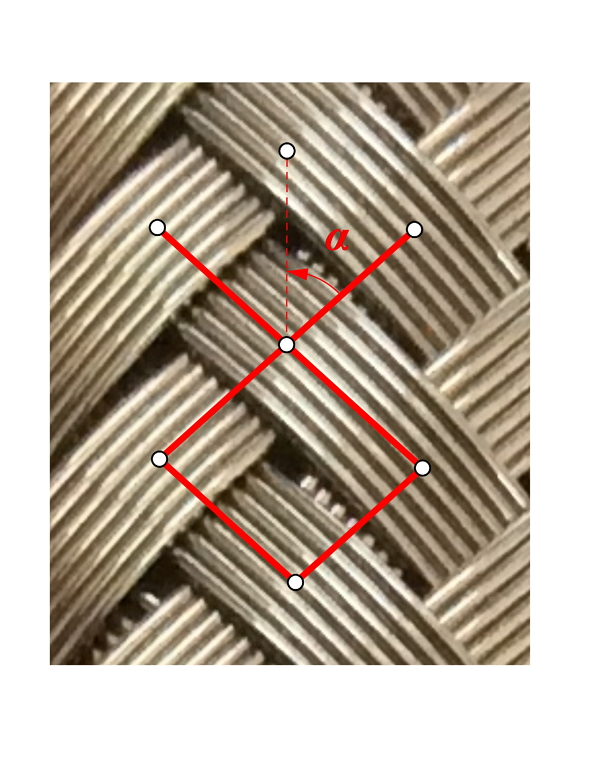
\includegraphics[width=0.7\linewidth]{figures/braid-angle}
\caption{ just have test}
\label{fig:braid-angle}
\end{figure}









%% Appendix

%\appendix
%
%\section{Section in Appendix}
%\label{appendix-sec1}








%% References
%%
%% Following citation commands can be used in the body text:
%% Usage of \cite is as follows:
%%   \cite{key}         ==>>  [#]
%%   \cite[chap. 2]{key} ==>> [#, chap. 2]
%%
\citeyear{Einstein}
%% References with bibTeX database:

%\bibliographystyle{elsarticle-num}
 \bibliographystyle{elsarticle-harv}
% \bibliographystyle{elsarticle-num-names}
% \bibliographystyle{model1a-num-names}
% \bibliographystyle{model1b-num-names}
% \bibliographystyle{model1c-num-names}
% \bibliographystyle{model1-num-names}
% \bibliographystyle{model2-names}
% \bibliographystyle{model3a-num-names}
% \bibliographystyle{model3-num-names}
% \bibliographystyle{model4-names}
% \bibliographystyle{model5-names}
% \bibliographystyle{model6-num-names}

\bibliography{sample}



\end{document}

%%
%% End of file `elsarticle-template-num.tex'.
